\chapter{Segundo Projeto: Sistema para Locação de Mídias}\label{cap:segundoProjeto}
\epigraph{``\textit{Com organização e tempo, acha-se o segredo de fazer tudo e bem feito}''.}{Pitágoras}

\lettrine[lines=4, lhang=0.1, lraise=0, loversize=0.2, findent=0.1em]{\textcolor{corTema}{N}}{ESTE} capítulo aplicaremos o conhecimento adquirido até o momento na construção de uma aplicação Web em Java totalmente funcional, terminando o desenvolvimento do sistema de locação de DVDs começado no capítulo~\ref{cap:primeiroProjeto}, alterando diversas coisas que já foram feitas, inserindo a possibilidade do cadastro de mídias de vários tipos e, enfim, a locação de uma ou mais mídias por cada cliente. Sim, eu sei que locadora de DVDs, BluRays etc. não são mais tão populares, mas acredito que você saiba o que são e é um bom exemplo para podermos colocar o que sabemos em prática.


\section{Introdução}

Assim como no capítulo~\ref{cap:primeiroProjeto}, neste capítulo será apresentada uma série de requisitos, de forma muito simplificada, que deve ser usada para criar uma aplicação Web da mesma forma que fizemos no capítulo~\ref{cap:sistemaVendaProdutos}. Novamente, tudo que será requisitado estará baseado no que já aprendemos, sendo assim, todas as funcionalidades requeridas poderão ser implementadas com recursos já vistos no capítulo~\ref{cap:sistemaVendaProdutos}, mas isso não implica que você não terá que se virar de alguma forma para resolver algum problema. Agora você está apto a desenvolver um sistema completo de locação de mídias usando tudo que aprendeu até o momento. Vamos lá?


\section{Apresentação dos Requisitos}

Você foi contratado para criar um sistema para controle de cadastro de mídias. Esse sistema irá manter o cadastro dessas mídias e permitirá que clientes as aluguem. O DER do banco de dados pode ser visto na Figura~\ref{fig:cap09DER}. Para gerar a base, com o MariaDB/MySQL em execução, abra o modelo da base no MySQL Workbench, disponibilizado nos arquivos do capítulo. Com o modelo aberto, clique no menu \destaque{\textit{Database}} escolha a opção \destaque{\textit{Forward Engineer...}} e siga o assistente. A base de dados, as tabelas e os relacionamentos serão criados, e serão feitas várias inserções em todas as tabelas, com exceção das de locação e de itens de locação.

\FloatBarrier
\begin{figure}[!htbp]
    \centering
    \caption{DER da base de dados}
    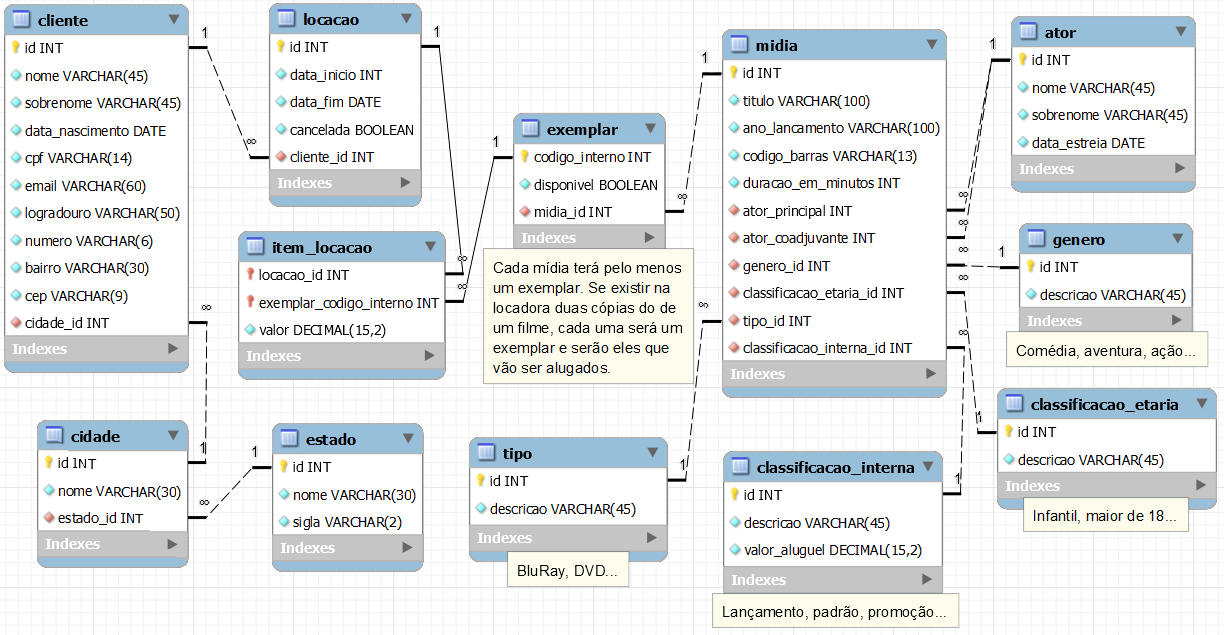
\includegraphics[scale=0.45]{imagens/cap09DER}
    \\\textbf{Fonte:} Elaborada pelo autor
    \label{fig:cap09DER}
\end{figure}
\FloatBarrier

As entidades e seus atributos você poderá ver no diagrama apresentado na Figura~\ref{fig:cap09DER}. Cada um dos cadastros base, ou seja, cadastro de mídias e seus exemplares, atores, gêneros, classificações etárias, tipos, classificações internas, clientes, cidades e estados, deve conter as funcionalidades de criar, alterar e excluir um determinado registro. A página principal da aplicação deve conter um \textit{link} para cada tipo de cadastro. Cada mídia pode ter um ou mais exemplares. O valor da locação virá da classificação interna de uma mídia, por exemplo, quando um filme ou jogo é lançamento, a locação é mais cara, concorda? Abaixo de cada nova tabela há uma caixa de texto com alguns exemplos do que poderia haver naquele cadastro para que você possa se guiar. O processo de locação é análogo ao processo de venda de produtos do capítulo~\ref{cap:sistemaVendaProdutos} e aqui a locação é por exemplar, então a tabela de itens de locação já está correta para a modelagem da solução desse problema, pois não será possível alugar o mesmo exemplar duas vezes na mesma locação.


\section{Desenvolvimento do Projeto}

O projeto ``LocacaoMidias'' já está disponível na pasta de projetos deste capítulo com uma implementação inicial. Abra-o no NetBeans e utilize-o como ponto de partida. As bibliotecas necessárias (JSTL, JSON e Validator) já estão configuradas no projeto, da mesma forma que foi feito no capítulo~\ref{cap:sistemaVendaProdutos}. A base de dados deve ter o nome de ``\texttt{locacao\_midias}'' e pode ser gerada a partir do modelo disponibilizado nos arquivos do capítulo, conforme descrito na seção anterior.

Com o projeto aberto, cabe a você terminar de desenvolver as funcionalidades que estão faltando: o cadastro de atores, o cadastro de mídias, o cadastro de exemplares e, a principal delas, o cadastro e a realização de locações. Sinta-se à vontade para personalizar os estilos, mudar cores, adicionar imagens ou qualquer outro artifício que julgar interessante para deixar a aparência da aplicação com a sua cara. Você pode, é claro, implementar tudo do zero se preferir.


\section{Resumo}

Neste capítulo foi requisitado que você implementasse uma aplicação Web em Java para gerenciar a locação de mídias como BluRays e DVDs, por isso, não há atividades a serem realizadas.
